\chapter{Ensayos y resultados}

\label{cap:EnsayosResultados}

En este capítulo se describe la fase de investigación previa al desarrollo del dispositivo de captura, junto con las pruebas realizadas para validar su correcto funcionamiento, tanto en un entorno de laboratorio como en una formación de Trenes Argentinos.

\section{Capturas del tráfico de la red en una formación}
\label{sec:capturas}

Como parte de la etapa de investigación, se realizaron visitas a los talleres de Trenes Argentinos en Victoria y Castelar, coordinadas respectivamente por Sergio Dieleke (Laboratorio Electrónico, Subgerencia de Material Rodante Línea Mitre) y Bruno Pilato (Laboratorio de Electrónica de Castelar, Línea Sarmiento).
El objetivo principal de estas visitas fue tomar capturas del tráfico del bus MVB, para ganar conocimiento acerca del estándar TCN y de la implementación particular en las EMU de Trenes Argentinos.

Para tomar las capturas se conectó un MAX485 y un analizador lógico VKTECH entre dos dispositivos MVB.
Se utilizó una PC para controlar el VKTECH y almacenar las diferentes capturas.
También se utilizó un osciloscopio para verificar que la señal capturada tuviera las características esperadas.
En la figura~\ref{fig:banco-capturas} se muestra un diagrama de bloques del banco de medición.
En las figuras~\ref{fig:foto-banco-capturas} y \ref{fig:osciloscopio} se muestra una fotografía del banco de medición y un detalle de la señal capturada en el osciloscopio.

% video con la secuencia https://drive.google.com/drive/folders/1I-V33ElLX13Iy0YliUeojRwYFQKuucAO
\begin{figure}[htbp]
	\centering
    {
        \fontfamily{phv}
        \fontsize{9pt}{9pt}\selectfont
        \input{./Figures/banco-captura.pdf_tex}
    }
	\caption{Banco de medición utilizado para tomar las capturas.}
    \label{fig:banco-capturas}
\end{figure}

\begin{figure}[htbp]
	\centering
	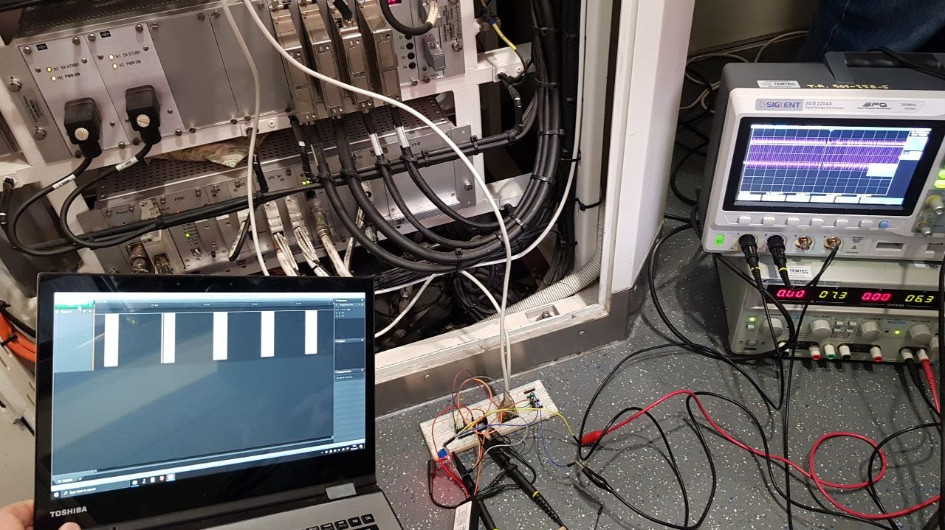
\includegraphics[width=\textwidth]{./Figures/foto-capturas.jpg}
	\caption{Fotografía del banco de medición utilizado para tomar las capturas.}
    \label{fig:foto-banco-capturas}
\end{figure}

\begin{figure}[htbp]
	\centering
	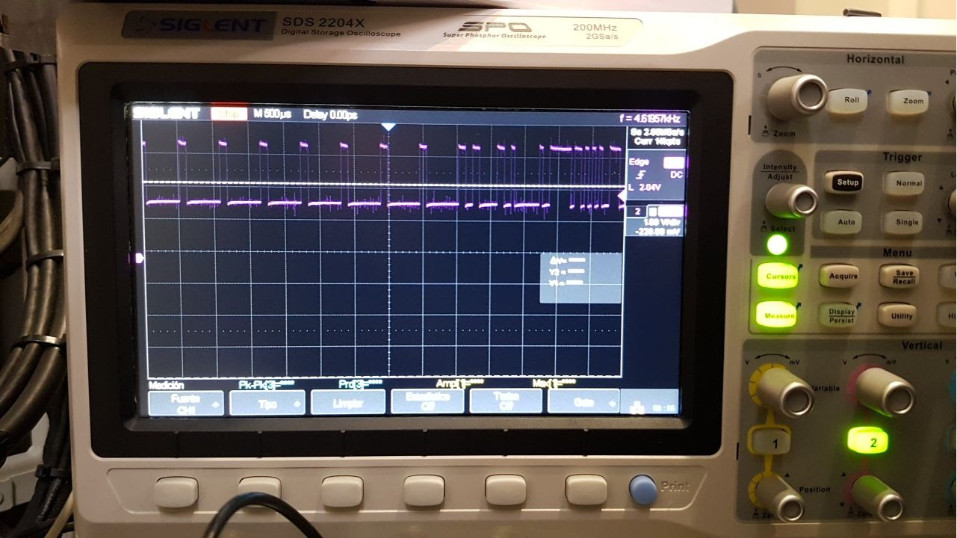
\includegraphics[width=\textwidth]{./Figures/osciloscopio.jpg}
	\caption{Señal MVB capturada en el osciloscopio.}
    \label{fig:osciloscopio}
\end{figure}

Se tomaron varias capturas de un minuto de duración del tráfico del bus MVB, con el banco de medición conectado en diferentes puntos del segmento.
En simultáneo con las capturas se efectuó el procedimiento de encendido de la red y una secuencia de pasos tales como tomar cabina, abrir y cerrar puertas, cambio de marcha, etc., de forma tal de generar tráfico en la red y así poder analizar en detalle el funcionamiento de la misma.

En la figura~\ref{fig:pulseview} se muestra una visualización de una de las capturas.
En la parte superior se observa que en los primeros 10 ms se transmitieron 10 telegramas, aunque el nivel de detalle no es suficiente para discernir el formato de las tramas.
En la parte inferior se amplía la visualización de uno de los telegramas, donde se puede apreciar en detalle las tramas \textit{master} y \textit{slave}.
Estas visualizaciones se obtuvieron utilizando el software PulseView, que es parte del proyecto Sigrok.

\begin{figure}[htbp!]
	\centering
    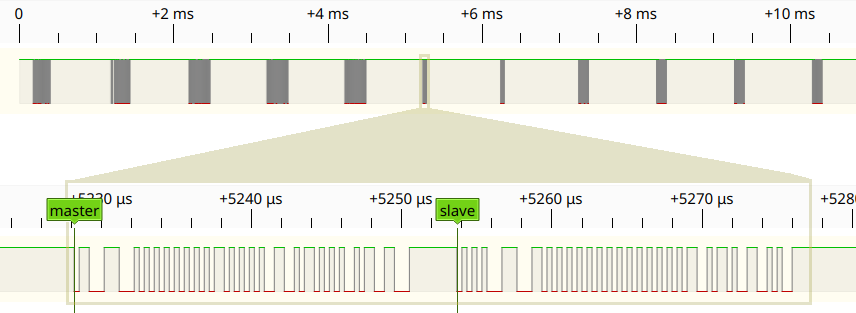
\includegraphics[width=\textwidth]{./Figures/pulseview.png}
    \caption{Visualización de una de las capturas realizadas.}
    \label{fig:pulseview}
\end{figure}

\section{Decodificación de las capturas}
\label{sec:decodificacion}

El siguiente objetivo en la etapa de investigación fue decodificar la información de las tramas capturadas. Para ello se desarrolló un programa en lenguaje Python que toma como entrada una captura en formato binario (un byte por muestra, como se describe en la sección \ref{sec:software}) y produce como salida un reporte de la información decodificada.

El software se compone de dos programas. El primero de ellos, \texttt{mvb\_signal.py}, toma como entrada una captura en formato binario, decodifica los datos codificados en Manchester, y produce como salida un archivo en formato CSV en el que cada línea representa un telegrama y tiene la forma \texttt{<tiempo>,\allowbreak <master>,\allowbreak <slave>}, donde \texttt{<tiempo>} es la marca de tiempo en segundos del telegrama, y \texttt{<master>} y \texttt{<slave>} es el contenido de las tramas en formato hexadecimal, sin incluir los delimitadores y las secuencias de verificación. En el código~\ref{cod:mvbsignal} se muestra un ejemplo de ejecución, en el que se procesa una captura que contiene 4 telegramas.

\begin{lstlisting}[label=cod:mvbsignal,caption=Ejemplo de ejecución de \texttt{mvb\_signal.py}.,float=htbp]
$ python3 mvb_signal.py < captura1.bin
0.0001,4390d6,971e0000008214
0.0011,431bf7,30000f
0.0021,000134,971e07
0.0022,4010c5,04004830580048
\end{lstlisting}

La salida de \texttt{mvb\_signal.py} se puede redireccionar mediante un \textit{pipe} al segundo programa, \texttt{mvbparse.py}, que interpreta la información de las tramas según el protocolo MVB y produce un reporte de la evolución de cada una de las variables identificadas. En el código~\ref{cod:mvbparse} se muestra un ejemplo de ejecución de \texttt{mvbparse.py}.

\begin{lstlisting}[label=cod:mvbparse,caption=Ejemplo de ejecución de \texttt{mvbparse.py}.,float=htbp,basicstyle=\footnotesize\ttfamily]
$ python3 mvb_signal.py < captura2.bin | python3 mvbparse.py
 [[port='0x31b'] [n=   12] [
                  t=  0.001s  0x30000f0c0110000000000000000011a8]],
 [[port='0x353'] [n=    3] [
                  t=  0.212s  0xe2036aa0000000000
                  t=  0.471s  0xe2036ba0000000000
                  t=  0.730s  0xe2036da0000000000]],
\end{lstlisting}

La salida de ejemplo de \texttt{mvbparse.py} indica que se identificaron dos variables, en los puertos \texttt{0x31b} y \texttt{0x353}.
La primera variable fue transmitida en total 12 veces, con un valor de 16 bytes. Se transmitió por primera vez en la marca temporal $0{,}001$ s, con un valor de 16 bytes, y luego se transmitió 11 veces más con el mismo valor.
La variable en el puerto \texttt{0x353} fue transmitida en total 3 veces con un valor de 8 bytes diferente cada vez.

Dado que durante la captura se realizaron diferentes acciones según se mencionó en la sección \ref{sec:capturas} (tomar cabina, abrir y cerrar puertas, etc.), fue posible, analizando la salida producida por el programa, detectar cuáles son las variables que cambian en función del momento en que estas acciones fueron efectuadas. En la figura~\ref{fig:analisis-captura} se muestra, por ejemplo, que la variable en el puerto \texttt{0x1b2} se modifica cada vez que se realizan las acciones de tomar cabina, y seleccionar, abrir y cerrar las puertas.

\begin{figure}[htbp]
	\centering
	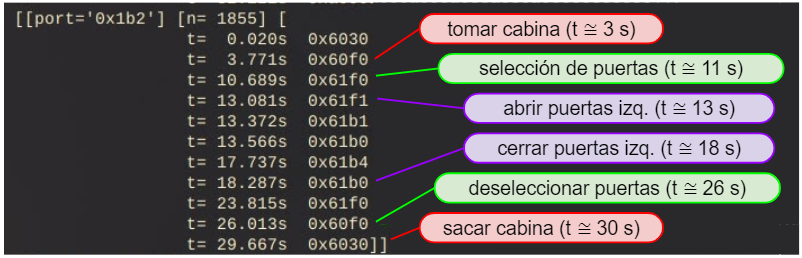
\includegraphics[width=\textwidth]{./Figures/analisis-captura.png}
	\caption[Resultado del análisis de una de las capturas.]{Resultado del análisis de una de las capturas.}
    \label{fig:analisis-captura}
\end{figure}

El software de decodificación está disponible en la plataforma Github \cite{mvbparse-py}. El desarrollo de este prototipo no solo sirvió para proporcionar información valiosa acerca del funcionamiento del bus MVB en las formaciones de Trenes Argentinos, sino también brindó la experiencia necesaria para el posterior desarrollo del software de captura descripto en la sección \ref{sec:software}.

\section{Pruebas del dispositivo de captura}

A continuación se describen los diferentes tipos de pruebas efectuadas para verificar el correcto funcionamiento del dispositivo de captura.

\subsection{Prueba del software de captura}

Para probar el correcto funcionamiento del software de captura (descripto en la sección \ref{sec:software}) se utilizaron las capturas tomadas en la formación ferroviaria (ver sección \ref{sec:capturas}).

Para ejecutar esta prueba se ejecuta el software pasándole como entrada el contenido de una de las capturas en lugar del flujo de datos en tiempo real. Para ello, en una consola se crea un FIFO y se lo alimenta con el contenido de la captura en un ciclo infinito. Se utiliza el comando \texttt{pv} \cite{pv} para limitar el ancho de banda a 12 MB/s:

\begin{lstlisting}
$ mkfifo /tmp/fifo
$ while cat captura.bin; do :; done | pv -L 12M > /tmp/fifo
\end{lstlisting}

En otra consola se ejecuta el software de captura tomando el FIFO como entrada.

\begin{lstlisting}
$ go run cmd/main.go </tmp/fifo
\end{lstlisting}

Esta técnica permite utilizar el software en una PC, como si estuviera conectado al bus MVB.
De esta manera se pudo probar todas sus funcionalidades, tanto en el modo interactivo como en el modo de captura.

\subsection{Prueba de integración de hardware}

% 28 oct 2021?
% 24 nov 2021?

El siguiente paso fue efectuar una prueba de integración del software de captura recibiendo el flujo de datos del VKTECH en tiempo real.
Para ello se utilizó el generador de señal MVB descripto en la sección \ref{sec:generador}, en una configuración como se muestra en la figura~\ref{fig:generador}.
En la figura~\ref{fig:educiaa+vktech} se muestra el banco de medición utilizado en esta prueba.

Esta prueba permitió verificar que es posible utilizar el VKTECH para recibir el flujo de datos en tiempo real.
La prueba se realizó con el software de captura corriendo tanto en una PC como en una Raspberry Pi.

\begin{figure}[htbp]
	\centering
	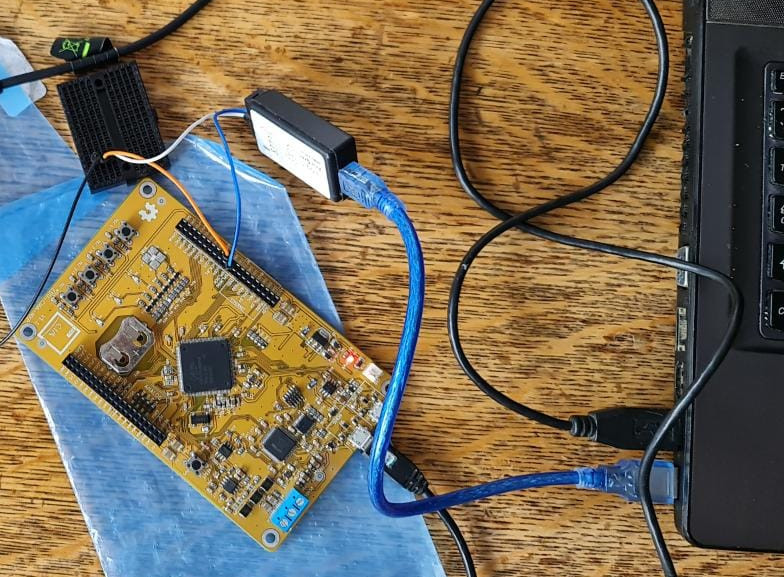
\includegraphics[width=\textwidth]{./Figures/educiaa+vktech.jpg}
	\caption{Banco de medición de la prueba utilizando el generador de señal MVB.}
    \label{fig:educiaa+vktech}
\end{figure}


\subsection{Prueba en una formación ferroviaria}

% 3 dic 2021 (PC)

% 6 ene 2022? (RPI)

La última prueba que se efectuó fue con el dispositivo de captura conectado en el bus MVB en una formación de Trenes Argentinos, como se muestra en la figura~\ref{fig:conexion}.
Se verificó que la conexión del dispositivo de captura no afectó al correcto funcionamiento del resto de los dispositivos conectados en el bus MVB. Sin embargo, cabe destacar que esta prueba se realizó en una formación detenida.
En la figura~\ref{fig:disp-captura} se muestra el dispositivo de captura, y en la figura~\ref{fig:disp-captura-ssh} se muestra una foto de la pantalla de una PC conectada mediante el protocolo SSH a la Raspberry Pi, en la que se captura el tráfico MVB en tiempo real.

\begin{figure}[htbp]
	\centering
	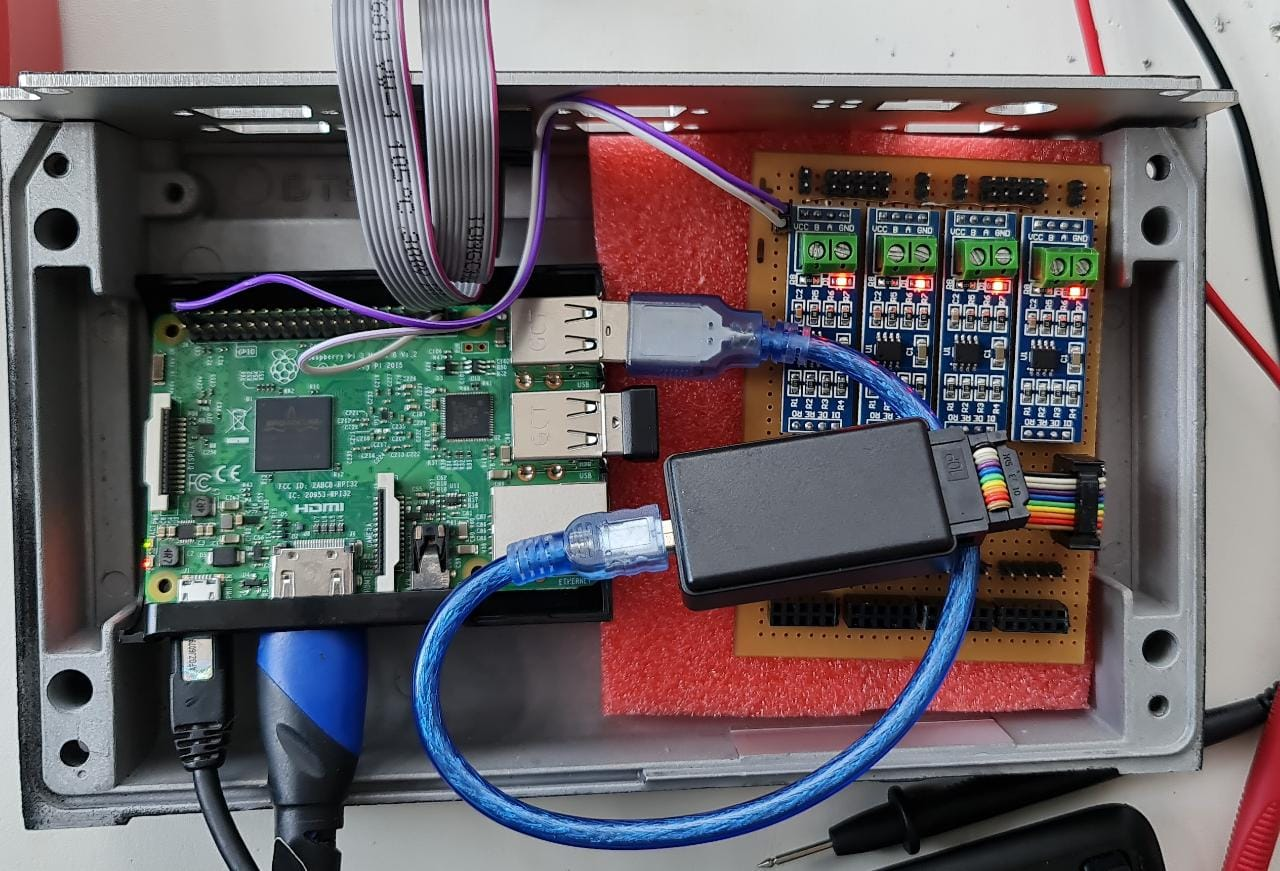
\includegraphics[width=\textwidth]{./Figures/disp-captura.jpg}
	\caption{Fotografía del dispositivo de captura.}
    \label{fig:disp-captura}
\end{figure}

\begin{figure}[htbp]
	\centering
	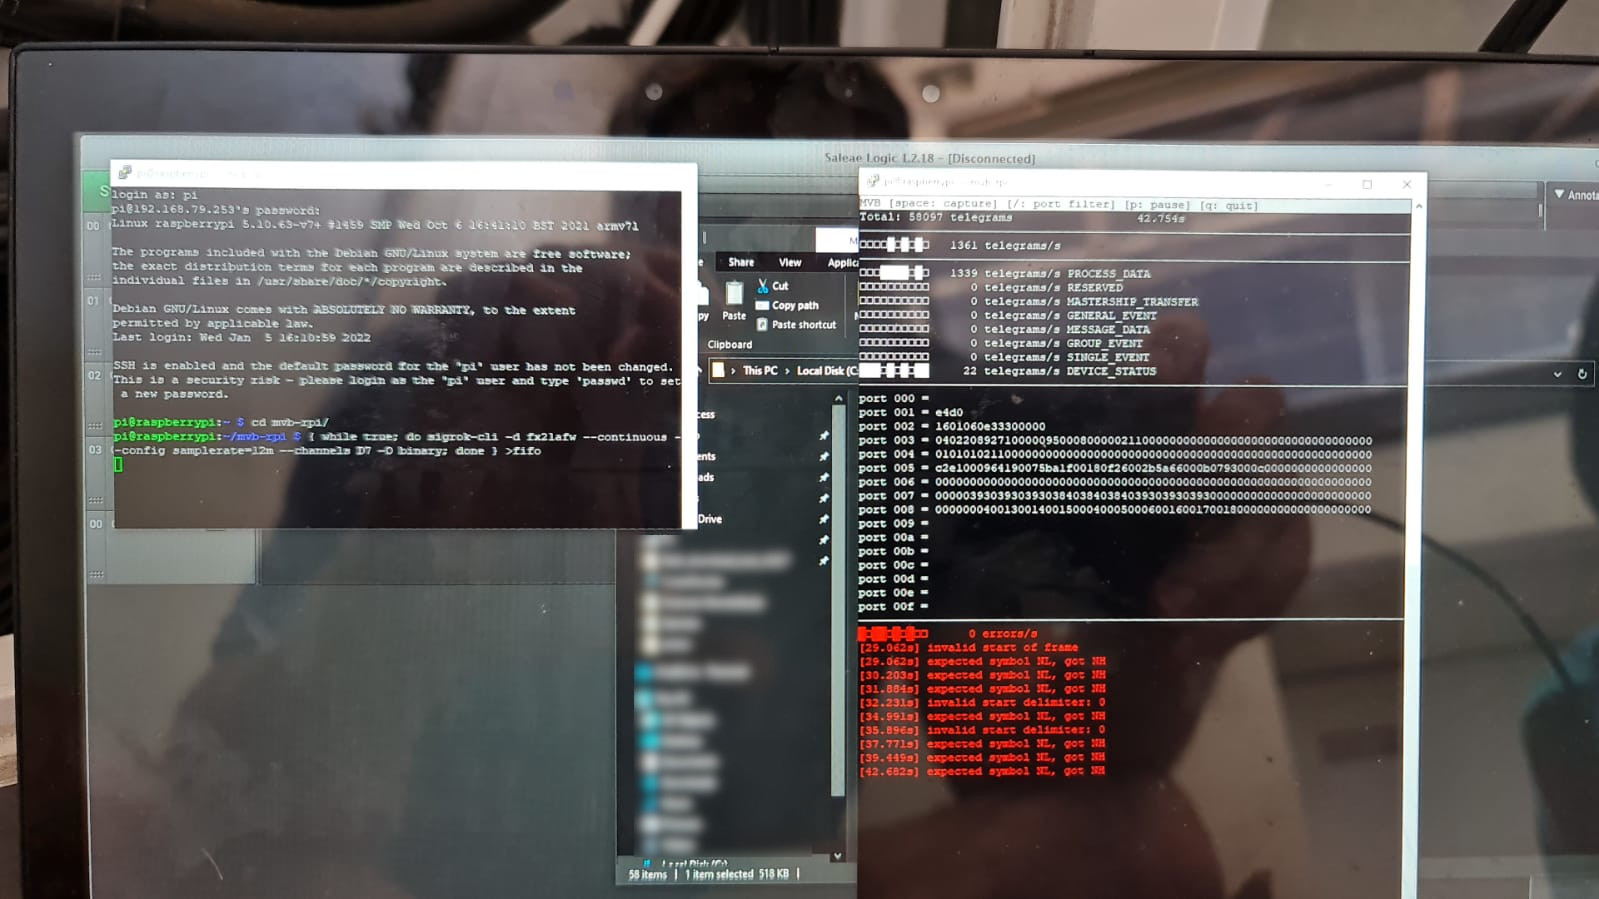
\includegraphics[width=\textwidth]{./Figures/disp-captura-ssh.jpg}
	\caption{Sesión de prueba del dispositivo de captura.}
    \label{fig:disp-captura-ssh}
\end{figure}
